%%%%%%%%%%%%%%%%%%%%%%%%%%%%%%%%%%%%%%%%%
% Short Sectioned Assignment
% LaTeX Template
% Version 1.0 (5/5/12)
%
% This template has been downloaded from:
% http://www.LaTeXTemplates.com
%
% Original author:
% Frits Wenneker (http://www.howtotex.com)
%
% License:
% CC BY-NC-SA 3.0 (http://creativecommons.org/licenses/by-nc-sa/3.0/)
%
%%%%%%%%%%%%%%%%%%%%%%%%%%%%%%%%%%%%%%%%%

%----------------------------------------------------------------------------------------
%  PACKAGES AND OTHER DOCUMENT CONFIGURATIONS
%----------------------------------------------------------------------------------------

\documentclass[norsk]{article} % A4 paper and 11pt font size

\usepackage[T1]{fontenc} % Use 8-bit encoding that has 256 glyphs
\usepackage{fourier} % Use the Adobe Utopia font for the document - comment this line to return to the LaTeX default
\usepackage[english]{babel} % English language/hyphenation
\usepackage{amsmath,amsfonts,amsthm} % Math packages

% Added by Joergen %---------------------------------------------------------------------
%\usepackage{cleveref}

% Added by Haavard %---------------------------------------------------------------------
\usepackage[utf8]{inputenc} % Norwegian letters
\usepackage{fullpage}
\usepackage{subcaption}
\usepackage[font={small, it}]{caption} % captions on figures and tables
\usepackage{graphicx}
\usepackage{color}
\usepackage{hyperref} % Use \autoref{ and \nameref{
\hypersetup{backref,
colorlinks=true,
breaklinks=true,
%hidelinks, %uncomment to make links black
linkcolor=blue,
urlcolor=blue,
citecolor=blue
}
\usepackage[all]{hypcap} % Makes hyperref jup to top of pictures and tables
% --------------------------------------------------------------------------------------

\usepackage{lipsum} % Used for inserting dummy 'Lorem ipsum' text into the template

\usepackage{sectsty} % Allows customizing section commands
\allsectionsfont{\centering \normalfont\scshape} % Make all sections centered, the default font and small caps

\usepackage{fancyhdr} % Custom headers and footers
\pagestyle{fancyplain} % Makes all pages in the document conform to the custom headers and footers
\fancyhead{} % No page header - if you want one, create it in the same way as the footers below
\fancyfoot[L]{} % Empty left footer
\fancyfoot[C]{} % Empty center footer
\fancyfoot[R]{\thepage} % Page numbering for right footer
\renewcommand{\headrulewidth}{0pt} % Remove header underlines
\renewcommand{\footrulewidth}{0pt} % Remove footer underlines
\setlength{\headheight}{13.6pt} % Customize the height of the header

\numberwithin{equation}{section} % Number equations within sections (i.e. 1.1, 1.2, 2.1, 2.2 instead of 1, 2, 3, 4)
\numberwithin{figure}{section} % Number figures within sections (i.e. 1.1, 1.2, 2.1, 2.2 instead of 1, 2, 3, 4)
\numberwithin{table}{section} % Number tables within sections (i.e. 1.1, 1.2, 2.1, 2.2 instead of 1, 2, 3, 4)

\setlength\parindent{0pt} % Removes all indentation from paragraphs - comment this line for an assignment with lots of text

%----------------------------------------------------------------------------------------
%  TITLE SECTION
%----------------------------------------------------------------------------------------

\newcommand{\horrule}[1]{\rule{\linewidth}{#1}} % Create horizontal rule command with 1 argument of height

\title{  
\normalfont \normalsize 
k\textsc{NTNU 2015} \\ [25pt] % Your university, school and/or department name(s)
\horrule{0.5pt} \\[0.4cm] % Thin top horizontal rule
\huge Project Notes\\ % The assignment title
\horrule{2pt} \\[0.5cm] % Thick bottom horizontal rule
}

\author{Jørgen Vågan \\ Supervisor: Ingve Simonsen} % Your name

\date{\normalsize\today} % Today's date or a custom date


\begin{document}


\maketitle % Print the title

%----------------------------------------------------------------------------------------
%  Text Body:
%----------------------------------------------------------------------------------------

%\listoftodos{}

\abstract{ Abstract..
abstract.}

\newpage
\section{Plasmons}
Notes from Justin White 
http://large.stanford.edu/courses/2007/ap272/white1/

\textbf{Surface Plasmon Polaritons}
\begin{itemize}
\item
Surface Plasmon polaritons are collective longitudinal oscillations
of electrons near a material surface, strongly coupled to 
an electromagnetic wave.

\item 
Both bulk and surface plasmons have associated EM-waves, and can
consequently be described by Maxwell's equations. 

\item 
the coherent oscillations of electron motion can be encapsulated in
the dielectric constant of the material. 

\item
The basic form of the bulk and surface plasmon solutions are shown
below:
\begin{align}
E_{bulk} &= E_0 e^{k_x x - \omega t}\\
E_{spp} &= E_0e^{-\kappa |z|} e^{k_x x - \omega t}
\end{align}
The bulk plasmons are associated with purely transverse EM waves
($E\perp k$ and  $B \perp k$) and can only exist for 
$\omega < \omega_p$. 
For $\omega > \omega_p$: the wave-vector for bulk plasmons becomes
imaginary, giving an exponentially decaying wave, instead of a 
propagating wave. It is for this reason that most metals 
are highly reflective for visible light ($\omega <\omega_p$),
but transparent for ultraviolet light ($\omega > \omega_p$)

\item
Surface plasmons have an associated EM wave with both transverse 
and longitudinal field components. Such waves can only be excited
at the interface between a conductor and dielectric, and aretightly bound to the surface. The field reach their maximum at the interface 
($z=0$), and exponentially decay away from the surface.

\item 
The wave-vector of the surface plasmon mode $k_{spp}$ always lies
to the right of the free space wave-vector $k_0$ (in the dispersion 
diagram/relation), such that $\lambda_{spp} < \lambda_0$. this makes
 it impossible to directly launch a surface plasmon wave by
illumination with free-space radiation, because the free-space photons
simply do not have enough momentum to excite the surface plasmon.

As $\omega$ increases, $k_{spp}$ gets larger and larger, moving
further  away from $k_0$ (textit{??making it harder and harder 
for light to excite the surface plasmons??})d. As $k_{spp}$ increases,
the surface plasmon wave is more tightly bound to the surface.
This process has an upper limit of $\omega_{sp}$, the surface 
plasmon resonant frequency, which occurs when the dielectric 
constant of the metal and the dielectric have the same 
magnitude but opposite signs.

\item
\textbf{Excitation of Surface Plasmons}\\
High energy electrons that bombard a thin metalic film can
launch surface plasmons and a surface plasmons of a whole range
of wavelengths can be excited. However, only plasmons
far along the dispersion curve, where $k_{spp}$ is largest
are generally excited.
\\
\\
As mentioned previously, direct excitation of surface plasmons by 
free-space photons is not achievable because $k_{spp}$ is 
always greater than $k_0$; this can be seen from the dispersion
relation, where the surface plasmon dispersion relation always
lies to the right of the free space dispersion curve.\\
This can be overcome by back-side illumination through a material
with a higher index of refraction $n$, where the far field radiation
has a larger wave-vector ($k=nk_0$) 
(like done in a Kretschmann-Raether coupler) [5].
A surface plasmon will be efficiently excited when 
\begin{align}
k_{\parallel} = n k_0 \sin \theta = k_{spp}
\end{align}
A mor egeneral approach to launch surface plasmons with light
is the use of structured surfaces that are able to impart momentum
on the photon, enabling it to couple to the surface plasmon mode.
Anything from a single sub-wavelength disk or slit, to rectangular
or sinusoidal diffraction gratings are used for this type of coupling.
\textbf{A thorough overview of surface plasmon coupling 
and patterned and rough surfaces is given by Raether[6]}


\item Appendix: Derivation of Bulk and Surface Plasmons (see article).
\end{itemize}

Other Nice sources:
\begin{itemize}
\item Really nice article on Plasmons:\\
http://nanocomposix.com/pages/plasmonics

\item Article:\\
http://cdn.intechopen.com/pdfs-wm/44351.pdf

\item Surface Plasmon Theory(book?):\\
https://www.physik.hu-berlin.de/de/nano/lehre/Gastvorlesung%20Wien/Plasmonics%20Pitarke

\item Chemistry-blog:\\
http://www.chemistry-blog.com/2007/03/19/plasmonics-part-ii/

\item Mie theory: \\
http://www.orc.soton.ac.uk/publications/theses/1460T\_lnn/1460T\_lnn\_03.pdf
\end{itemize}




\newpage
\textbf{From Wikipedia}
\begin{itemize}
   \item \textbf{What are Plasmons?} \\
A plasmon is a quantum of plasma oscillation (quasiparticle from the quantization of plasma oscillations).
Plasmons are collective (a discrete number) oscillations of the free elctron gas density.
Plasmons can also couple with a photon to create another quasiparticle called a plasma polariton
(electromagnetic wave - electric/magnetic dipole-carrying exitation - coupling.
\\
\\
Plasmons can be described as oscillations of free elctron density with respect to
fixed positive ions in a metal. Imagine a cube of metal placed in an external 
electric field pointing to the right. Electrons will move the the left side and uncover
positive ions on the right side. The electrons will continue moving left until they
cancel the field inside the metal. Removing the field will make the electrons move back by their
mutual repulsion and attraction to the ions, leaving the electrons to oscillate back and forth,
at the \textbf{plasma frequency}, in a so called plasma oscillation.

\item \textbf{Plasma Oscillation, aka ''Langmuir waves''} \\
Rapid oscillations of electron density in conducting media such as plasmas or metals.
The oscillations can be described as an instability in the dielectric function of a free electron gas.
The frequency depends weakly on the wavelength of the oscillation.
\\
\\
'Cold' electrons (plasma oscillations)\\
If the thermal motion of the electrons is ignored and assuming infinite ion mass,
the charge density oscillates at the plasma frequency
\begin{align}
   \omega_{pe} &= \sqrt{\frac{n_e e^2}{m^* \varepsilon_0}}, \text{[rad/s] (SI-units)} \\
   \omega_{pe} &= \sqrt{\frac{4 \pi n_e e^2}{m^*}}, \text{(cgs-units)},
\end{align}
where $n_e$ is the number density of electrons, $e$ is the electric charge, $m^*$ is the effective mass of
the electron and $\varepsilon_0$ is the permittivity of free space. Since the frequency is independent of 
the wavelength, these oscillations have an infinite phase velocity and zero group velocity.
Note in addition that, if $m^*$ is the electron mass $m_e$, the plasma frequency $\omega_{pe}$
depends only on the physical constants and concentration of electrons $n_e$. The numeric expression is:
\begin{align}
f_{pe} = \frac{\omega_{pe}}{2 \pi} \approx 8980 \sqrt{n_e}, \text{[Hz]}
\end{align}
with $n_e$ in [cm$^{-3}$]
\\
\\
'Warm' electrons (plasma oscillations)\\
When the effects of the electron thermal speed $v_{e,th} = \sqrt{\frac{k_B T_e}{m_e}}$ are taken into account,
the electron pressure acts as an additional restoring force and the oscillations propagate with
frequency and wavenumber related by the longitudinal Langmuir wave:
\begin{align}
\omega ^2 = \omega_{pe} ^2 + \frac{3 k_B T_e}{m_e} k^2 = \omega_{pe} ^2 + 3k^2 v_{e,th}^2
\end{align}
called the 'Bohm-Gross dispersion relation'. If the spatial scale is large compared to
the Debye length (measure of a charge carrier's net electrostatic effect in solution, 
and how far those electrostatic effects persist), the oscillations are only weakly modified
by the pressure term, but at small scales the pressure term dominates and 
the waves become dispersionless with a speed of $\sqrt{3}v_{e,th}$. For such waves, however, the
electron thermal speed is comparable to the phase velocity, i.e.
\begin{align}
v \sim v_{p,th} \equiv \frac{\omega}{k},
\end{align}
so the plasma waves can accelerate electrons that are moving with speed nearly equal to the
phase velocity of the wave. This process often leads to a form of collisionless damping
called Landau damping. Consequently, the large-k portion in the dispersion relation is difficult to
observe and seldom of consequence.
\\
\\
In metal of semiconductor, the effect of the ions periodic potential must be taken into account. This is
usually done by using the electrons effective mass in place of $m$.

\item \textbf{Role of Plasmons} \\
Plasmons play a large role in the optical properties of metals. Light of frequencies below the
plasma frequency is reflected, because the electrons in the metal screen the electric field 
of the light. Light of frequencies above the plasma frequency is transmitted, because the
electrons cannot respond fast eneough to screen it. In mot metals, the plasma frequency is in the 
unltraviolet, making them shiny (reflective) in the visible range. 
In semiconductors, the valence electron plasma frquency is usually in the deep ultraviolet, which is why
they are reflective.
\\
The plasmon energy can often be estimated in the free electron model as
\begin{align}
   E = \hbar \sqrt{\frac{n_e e^2}{m^* \varepsilon_0}} = \hbar \omega_p
\end{align}




\item \textbf{Surface Plasmons (SPs)} \\
Surface plasmons (plasmons at the interface of two materials) interact strongly with light,
resulting in a polariton (usually occurs at metal or doped dielectric interface, 
which both have small Im($\varepsilon$) > 0 and big Re($\varepsilon$) < 0).
These surface electron oscillations can exist at the interface between
any two materials where the real part of the dielectric function changes sign across the interface
(e.g. a metal-dielectric interface like metal sheet in air).
\\
SPs have lower energy than \textbf{bulk (or volume)} plasmons, which quantise the longitudinal
electron oscillations about positive ion cores within the bulk of an electron gas (or plasma).
\\
\\
The charge motion in a surface plasmon always create electromagnetic fields outside (as well as inside)
the metal. The total excitation, including both the charge motion and associated electromagnetic field,
is called either a \textbf{surface plasmon polariton} at a planar interface, or a \textbf{localized
surface plasmon} for the closed surface of a small particle.
\\
\\
Surface Plasmon polaritons can be excited by electrons or photons. In the case of photons, it
cannot be done directly, but requires a prism, or a grating, or a defect on the metal surface.
\textit{??? Or like trunctated spheres on granular films???}.
\\
\\
At low frequency an SPP approaches the dispersionrelation in free space $\omega = ck$.
At high frequency, the dispersion relation reaches an asymptotic limit called the ''sufrace plasma frequency''.
\\
\\
As an SPP propagates along the surface, it loses energy to the metal
due to absorption and due to scattering into free-space or into other directions. The electric field
falls off evanescently perpendicular to the metal surface. At low frequencies, the SPP penetration depth into
the metal is commonly approximated using the 'skin depth formula'. In the dielectric, the field 
will fall off far more slowly. SPPs are very sensitive to slight perturbations within the skin depth and because of this, SPPs, are often sed to probe inhomogeneities of a surface
\\
\\
Surface plasmons have been used to control colors of materials and is possible since controlling 
the particle's shape and size determines the types of surface plasmons that can couple to it and 
propagate across it. This in turn controls the interaction of light with the surface.
These effects are illustrated by the historic \textit{stained glass} wich adorn medieval
cathedrals. In this case, the color is given by metal nanoparticles of a fixed size which interact
with the optical field to give the glass its vibrant color. To produce optical range surface plasmons
effects involves producing surfaces wich have features < 400nm.
\\
\\
Surface plasmons are very sensitive to the properties of the materials on which they propagate.


\item \textbf{Surface Plasmons Resonance (SPR)} \\
Surface plasmon resonance is the resonant oscillation of conduction electrons at the interface
between a negative and positive permittivity meterial stimulated by incident light. The resonance
condition is estalished when the frequency of incident photons matches the natural
frequency of surface electrons oscillating against the restoring force of positive nuclei.
\\
\\
Surface plasmon polaritons are surface electromegnetic waves that propagate in a direction parallel to
the metal/dielectric (or metal/valcuum) interface. Since the wave is on the boundary of the metal
and the external medium, these oscillations are very sensitive to any change of this boundary, such as
adsoption of molecules to the metal surface.
\\
\\
To describe the existence and properties of surface plasmon polaritons, one can choose from various models,
e.g. the \textbf{Drude Model}. The simplest way to approach the problem is to treat each
material as a homogeneous continuum, described by a frequency-dependent relative permittivity between 
the external medium and the surface (this is a complex dielectric function). In order
for the terms that describe the electronic surface plasmons to exist, the real part of the dielectric constant
of the metal must be negative and its magnitude must be greater than that of the dielectric.
This condition is met in the infrared-visible wavelength region for air/metal and water/metal interfaces (where
the real dielectric constant of a metal is negative and that of air or water is possitive).
\\
\\
Localized SPRs (LSPRs) are collective charge oscillations in metallic nanoparticles that
are excited by light. They exhibit enhanced near-field amplitude at the resonance wavelength.
This field is highly localiced at the nanoparticle and decays rapidly away from the nanoparticle/dielectric
interface into the dielectric background, though far-field scattering by the particle is also 
enhanced by the resonance. Light intensity enhancement is a very important aspect of LSPRs and
and localization means the LSPR has very high spatial resolution (subwavelength), lmited
only by the size of nanoparticles. Because of the enhanced field amplitude, effects that depend on the
amplitude such as magneto-optical effect are also enhanced by LSPRs.
\\
\\
In order to excite surface plasmoms in a resonant manner, one can use an electron or light beam
(visible and infrared are typical). The incoming beam has to match its momentum to that of the plasmon.\\
With p-polarization this is possible by assing the light through a block of glass to
increase the wavenumber (and the momentum) and achieve the resonance at a given wavelength and angle.\\
s-polarized light however cannot excite electronic surface plasmons.
\\
\\
When the surface plasmon wave interacts with a local particle or irregularity, such as a rough surface,
part of the energy can be re-emmited as light. This emitted light can be detected behind the metal film
from various diretions.


\item \textbf{The Drude Model}\\
Treats the behavior of electrons in a solid like a pinball machine. 
The electrons are small light balls in a sea of static, positively charged ions. The only 
form of action instantaneous collisions.


\item \textbf{Mie Scattering}\\
Mie theory is sometimes used for the collection of methods and solutions to Maxwell's equations
for scattering, by e.g. using geometries where one can write separate equations for the radial and angular
dependence of solutions. More broadly, ''Mie scattering'' suggests situations where the size of the
scattering particles is comparable to the wavelength of the light, rather than much smaller or much larger.
\end{itemize}

\begin{thebibliography}{9}

      \bibitem{} 

\end{thebibliography}


\newpage
\section{Article Notes}
\subsection{Thermochromism}
\cite{intelligentWindows} 
\textbf{Intelligent Themochromic Windows} \\
The use of air-conditioning systems to maintain comfortable working and 
living environments has become more common [1]. This leads to an increase in hte use
of electricity and a concurrent increase in carbon dioxide emmissions and other 
atmospheric pollutants formed in the electricity generation process. A self-propagating cucle results,
in which blobal warming due to increases in these greenhouse gases necessitates the increased 
use of air conditioning systems. Technology is thus required that can reduce the use of air conditioning
commercial and residential buildings to help break this cycle. \\
\\
(...) window coatings can reduce cooling costs or heating requirements [2]. 
Using thermochromic coatings as intelligent window coatings[1-7], which change
their optical properties with temperature; usually related to a structural pase change on passing through a 
critical temperature $T_c$. Thermochromic coatings would be applicable to climates where there are extreme 
changes in temperature over the year, for example, central and northern Europe, Japan, the United States, 
and Canada, which have hot summers and cold winters. \\
\\
Vanadium(IV) oxide; transition temperature $Tc = 68 ^{\circ}$C; visually and infrared trasnparent belov $T_c$ 
$\rightarrow$ solar radiation passes through, keeping the interior warm. Below $T_c$ it becomes infrared reflective
and preventing excessive heating, while remaining visually transparent.\\
\\
Critical temperature for vanadium is too high, but this can be lowered to $25^{\circ}$C uing dopants ([9]),
most efficiently with tungsten(loading of only 2 atom percent required), in thin films prepared by physical 
vapor deposition methods [10] and sol-gel spin or dip coating [11]. \\
\\
problem: low luminous transmittance of the glazing VO$_2$ film [10-13]. (could be solved with doping[4]
or anti-reflective coating ([12])). Also one needs a method where the thin films of the material
can be applied cheaply and efficiently to the glass ([17]).\\
\\
(p.394) Discussion of MST(metal-to-semiconductor transition) of VO$_2$ and structure 
changes through the MST. Discussion involves structure figures.\\
\\
Goodenough proposes antiferroelectric transition being the drivings force
for the MST in VO$_2$. $\rightarrow$ two transition temperatures: one due to antiferroelectric
distortion and one due to the crystallographic distortion. \\
\\
The next paragraph explains how doping of various elements varies the MST temperature. 
The most effective dopant in reducing the temperature is Tungsten (additional info about tungsten 
and after that it considers other dopants). \\
\\
Thinner thickness, stress and strain can also reduce the thermchromic transition temperature.\\
\\
A little bit on VO$_2$ thin film durability? \\
Methods of preparing Pure  and doped Vanadium(IV) Oxide Films:\\ 
Sol-Gel Method: forming thin films by dip- or spin-coating substrates with solutions of metal alkoxides. \\
PVD Method: energetically removing atoms/molecules under reduced pressure conditions, then to react with seed gas. \\ 
CVD method: chemical vapor deposition, in particular atmospheric pressure CVD (APCVD). \\
APCVD: deposit tin solid films from gaseous precursors onto a suitable substrate. (+Pictorial representation)\\
(and more on APCVD).\\
\\
Comparison of the above methods. \\
\\
3 atom percent tungsten(VI) $\rightarrow$ transition temperature reduced to $5^{\circ}$C.\\
1.9 percent $\rightarrow$ $29^{\circ}$C.\\
transition temperature decreases linearly with tungsten atom percent incorporation(Figure). \\
\\
Summary: intelligent TC glass with desired switch temperature($25-30^{circ}$C, obtainable using APCVD.
Mst of the problems regarding commercial use are solvable. Market in household, offices, factories and space
exploration.\\


\newpage
\cite{TCcommercialProducts} 
\textbf{Thermochromism in Commercial Products} \\
\begin{itemize}
\item Thermochromic liquid crystals: Periodicity between layers, PITCH, and constructive interference!. 
   TC liquid crystals can have a versatile range of colors and useful color changes bewteen -30 
   and 120$^{\circ}$C, often with very high temperature sensitivity. TC liquid crystals are only useful when
   they are in the liquid crystalline phase, which is a meso-phase (an intermediate phase of matter) between
   an isotropic liquid (high temperature) and crystalline solid (low temperature), which restricts the
   temperature range of theur applicability.
\item \textbf{Microencapsulation}: Defined as the coating of small solid particles, liquid droplets,
   or gas bubbles with a thin film or coating or shell material, and typical particle sizes are
   1 to 1000 $\mu$m ([20] Kirk-Othmer Encycloped. of chem. Tech. 4thEd). For three component organic mixtures,
   particle sizes are < 50 $\mu$m. \textbf{Micro encapsulation allows the additional advantage 
   of combinations of several narrow color ranges}, and very sharp color changes, 
      as well as protection of the coloring agent
   from the environment ([16] Nakasuji med flere. Chem.Abs.).
   \textbf{complex coacervation} and \textbf{interfacial polymerization} $\rightarrow$ processes to
   microencapsulate thermochromic materials! Also described! Nice to include if I use thin layer on my 
   granular film!
\item Smart window candidates: Fe$_3$O$_4$, FeSi$_4$, NbO$_2$, NiS, Ti$_2$O$_3$ and VO$_2$, which
   owe their temperature change to a semiconductor-to-metallic state transition 
   (aka \textbf{Mott transition temperature})
\end{itemize}



\newpage
\cite{TCqualitativeDescription} 
\textbf{A Qualitative Description of Thermochromism in Color Measurements} \\
\begin{itemize}
\item Wyszecki and Stiles stated ([2] color science), for TC transmitting filters, that the spectral
   transmittance curve at a given wavelength with a large positive slope usually dereases with increasing
   temperature. As a rule: steeper(positive) slope $\rightarrow$ greater temperature effect! \\
   The curve with negative slope is of minor importance, but often causes transmittance increase for
   increasing temperature (if it is important). \\
   \\
   Neutral samples (gray, white, black) did not exhibit TC, because their spectral reflectance curves
   have a small or no slope.
\item Assuming nonfluorescent, linear material which is "nice" with respect to polarization effects, then
   \begin{align*}
      1 = R_{\lambda} + A_{\lambda} + T_{\lambda}
   \end{align*}
   where, $R_{\lambda}$ is the reflectance, $A_{\lambda}$ is the absorbance and $T_{\lambda}$ is the
   transmittance of the sample.\\
   Considering \textbf{transmitting samples}, the intensity $I_{\lambda}$ transmitted through a 
   sample of thickness $d$ is given by
   \begin{align*}
      I_{\lambda} = I_{0 \lambda} e^{- \mu_{\lambda} d}
   \end{align*}
   where $\mu_{\lambda}$ is the absorption coefficient of the sample at wavelength $\lambda$.
   The optical density $D$ is then given by:
   \begin{align*}
      D = -\log(T_{\lambda}) = -\log(\frac{I_{\lambda}}{I_{0\lambda}}) = \mu_{\lambda} d \log e
      = \frac{\mu_{\lambda}}{\ln 10}
   \end{align*}
   For \textbf{opaque samples} there is no transmittance, but the optical density can be calculated
   from the reflected intensity $I_{R\lambda}$:
   \begin{align*}
      D_{\lambda} = -\log(\frac{I_{R\lambda}}{I_{0\lambda}}).
   \end{align*}
   The light reflected from the material is also exponentially attenuated, for opaque materials.
   Thus, $D=\frac{\mu_{\lambda}}{\ln 10}$ holds for reflected light if $d$ is the distance the
   reflected light has passed in the material.
\end{itemize}


\newpage
\cite{renewableSustainableEnergyRev}
\textbf{A Qualitative Description of Thermochromism in Color Measurements} \\
\begin{itemize}
\item
\end{itemize}

      
\newpage
\cite{Kamalisarvestani2013}
%\cite{coatingTechOfTCthinFilmSmartWindows}
\textbf{Performance, materials and coating technologies of thermochromic thin films on smart windows} \\
\begin{itemize}
\item A significant amount of energy is consumed to maintain thermal comfort in buildings, 
   a huge portion which is lost through windows. 
   smart windows obtained by thin films is the solution. The touchstone of performance 
   is the change in visible and infra-red transmission and reflectance!
\item A significant amount of the energy consumption in buildings are mainly due to HVAC (heating, ventilation 
   and air conditioning) devices, used to obtain thermal comfort,
   The building energy consumption in developed contries accounts for 20-40$\%$ of the total energy use.
   (including further details of US and China energy consumption). The building energy consumption is even more
   dominant in hot and humid regions, using one-third to half of the elextricity produced in some contries.
   Energy related carbon dioxide emmision. Motivates energy saving measures to reduce building energy losses and CO$_2$
   emissions.
\item Two approaches to increase energy efficieny (7-10)
   \begin{itemize}
      \item Active stratergies: improving HVAC systems and building lighting.
      \item Passive stratergies: improving the thermal properties of the building envelope (elementss
         separating the indoor from outdoor), i.e. thermal insulation to wall, cool coatings on roofs
                  and coated window glazings.
   \end{itemize}
\item Windows are known as one of the most energy inefficient components of buildings.(11) \\
      Improving the thermal performance of windows will result in reduced electricity costs 
      and less greenhouse gas emmissions. \\
      In addition to controlling transmitted IR radiation an ideal window should be capable 
      of sufficient transmission of visible light(12). \\
      Improving glazing characteristics of windows such as 
      thermal transmittance and solar parameters is the most 
      important criterion to be considered in building winows standards (14).
\item International and local standards related to energy and lighting performance of windows TABLE.
\item \textbf{Smart windows} defined as the type of windows that partially block the unwanted solar radiation.
   The energy performance can be improved by increasing heat gain in cold weather and 
   decreasing it in hot weather by adopting
   windows radiative and thermal properties dynamically (25). Adding a 
   controllable absorbig layer on teh surface of hte glass
   can change the optical properties of the glass by controlling the 
   incident solar heat flux(26). Therefore, smart windows
   lead to reduced HVAC.energy consumption, size and elecric demand of the building (11,27,28).\\
\item $\big($Low emissivity (low-E) coatings are spectrally selective films that are aimed to let the 
   visible light pass through and block the IR and UV-wavelengths which generally create heating(10).
   Typically, there are two types of these coatings: the tin oxide based hard coating and the 
   silver based soft coating with higher IR reflectance and lower transmittance. The visible transmittance
   of hard coatings can be boosted with anti-reflecting silicon dioxide (29). $\big)$
\item \textbf{The switchable reflective devices} (also called dynamic tintable windows) are categorized into
   \textbf{passive-} and \textbf{active systems}:
   \begin{itemize}
         \item Passive devices: the switching process is activated automatically in accordance 
            with the environmental conditions, e.g. temperature and heat in thermochromic windows.
         \item Actice systems: Require an external triggering mechanism to perform the modulation. For 
            instance, electricity is the actuating signal in electrochromic windows. The active
            switchable glazing systems offer supplementary options compared to the passive systems 
            whereas their dependenvy on power supply and wiring should be reckoned with as a drawback.
   \end{itemize}
\item Chromic material, liquid crystals and suspended particle windows are the three most common
   active controlled intelligent windows (11). 
   (Chromic materials $=$ electrochromic(active), gasochromic(active),
   photochromic and thermochromic.
\item Providing a see-through mode is a must in any application.
\item (p.356) The technology using liquid crystals in intelligent windows is called Polymer.
   Dispersed liquid crystals (PDLC).
\item Electrochromic windows and thermochromic windows demand the lowest cooling energy, where the former
   require less energy for lighting than the latter (69). \textbf{Figure 1 (24) (nice figure comparing 
   TC to the other chromic glazings together with clear glass, tinted glass and reflective glass) }.
\item \textbf{Thermochromic Windows}: \textbf{ALSO NOTE PAGE 357! ALOT OF NICE FIGURES!!!}\\
   Word originates from the Greek roots: "thermos" meaning warm or hot; and "Chroma" which means color.
   Generally TC materials change color in response to temperature variations.\\
   The TC thin film is initially in its monoclinic state(cold state) at lower temperatures (usually
   room temperature). Monoclinic materials behave as semiconductors, less reflective especially in 
   the near-IR (NIR) radiation. As the temperature becomes higher than a certain point, the TC material
   changes its nature from monoclinic to rutile state(hot state), where the material acts like a 
   semi-metal, reflecting a wide range of solar radiation (76). \textbf{FIGURE 3}
   The transition is called \textbf{metal to semiconductor transition (MST)}.
\item \textbf{Figure 4}, The majority of the heat gain in solar spectrum takes place at NIR range
   (800-1200 nm) (78-80). The red line(line 1) indicates the transmittance of a perfect
   TCW in cold state. Visible light should be transmitted and NIR should be reflected. Long wave radiation
   is also reflected back to indoor. This transmittance approach leads to reduction of solar heat gain and is 
   apt in nearly all climates. \\
   The blue line(line 2) indicates the tranmittance of a perfect TCW in its hot state. Visible
   and near infrared radiation are transmitted, while long-wave infrared is reflected to inside.
   This transmittance mode is suitable in low temperature climates where solar heat gain is desired.
   Therefore, in high temperatures, TCW reduce NIR and far-IR transmittance, while in low temperatures
   they allow these parts of solar adiation to pass (82), (Figure 5). \\
   The MST is fully reversible, co-occurred with large variations in electrical and optical 
   properties in NIR range (83). The MST temperature should decrease to near the ambient
   temperature. Doping metal ions into the lattice of TC materials can alter the transition temp(84,85).
   The size and charge (84,86,87) of dopant ion, film's strain (88,89) as well as the variations in
   electron carrier density are the determinant factors prevailing on the fall or rise of the transition
   temperature (90).
\item The \textbf{Ideal spectral behavior of TCW} is presented in \textbf{Table 3}. 
   %\begin{table}
      %\caption{The ideal optical performance of thermochromic windows (adapted from (91)).}
      %\hline
      %\textbf{State}    & \textbf{Monoclinic/cold (T<T_t)}    & \textbf{Rutile/hot (T>T_t)}    \\
      %\hline
       %Wavelength        & Visible   \t NIR  & Visible   \t NIR  \\
       %Transmittance (T) & 60\%-65\% \t 80\% & 60\%-65\% \t 15\% \\
       %Reflectance (R)   & 17\%      \t 12\% & 17\%      \t 77\% \\
      %\hline
   %\end{table}
   The visible transmission and reflectance should be equal on both sides of transition, 
   while the infra-red variations
   are from $0\%$ to $65\%$. The change in transmittance ($\Delta T \% $) and reflectance ($ \Delta R \% $)
   can be formulated as (92):
   \begin{align*}
   \Delta T \% &= ( T_{hot} - T_{cold} ) \cdot 100 \\
   \Delta R \% &= ( R_{hot} - R_{cold} ) \cdot 100
   \end{align*}
   where hot and cold denotes transmittance/reflectance at the hot and cold state respectively.
\item The most common TC material in TCWs is pure \textbf{vanadium dioxide}, with a transition temperature of
   $68  ^{\circ}$C which shoud be decreased to ambient temperature for practical use.\\
   The most critical weakness of VO$_2$ coatings is their low transmittance in the visible range.
   Many studies have reported values between $40 \%$ and $50 \%$, which is well below the acceptable
   value of $60 \%$ (93, 94). \textbf{Table 4} shows the reported values of transmittance and reflectance
   in the visible and IR range for VO$_2$.
\item Low energy-saving efficiency also limits the application of VO$_2$ coatings. The
   change in transmittance before and after the transmittion temperature $T_t$, at 2500nm, is
   known as the \textbf{switching efficiency} $\eta_T$ and is the benchmark of energy-saving efficiency.
   (?why? because of lighting?). This value is incluenced by doping(107,108), microstructure(80,95,109-111),
   \textbf{and film thickness (80,88)}. The most paramount factor among them is film thickness that affects
   the switching efficiency most significantly. However, increasing the film thickness has an adverse
   effect on $T_{vis}$. As observed from table 4, \textbf{the ideal film thickness is between 40 and 80 nm}.
\item Crucial Steps to overcome the limited application of TWCs:
   \begin{itemize}
      \item Suitable doping(reducing $T_t$ and improving $T_{vis}$)
      \item Appropriate Coating Technology
      \item Adding efficient anti-reflecting coating(to increase $T_{vis}$) (read next title in article)
      \item Reducing coating costs
   \end{itemize}



      
\end{itemize}

\begin{figure}[h!]
  \centering
   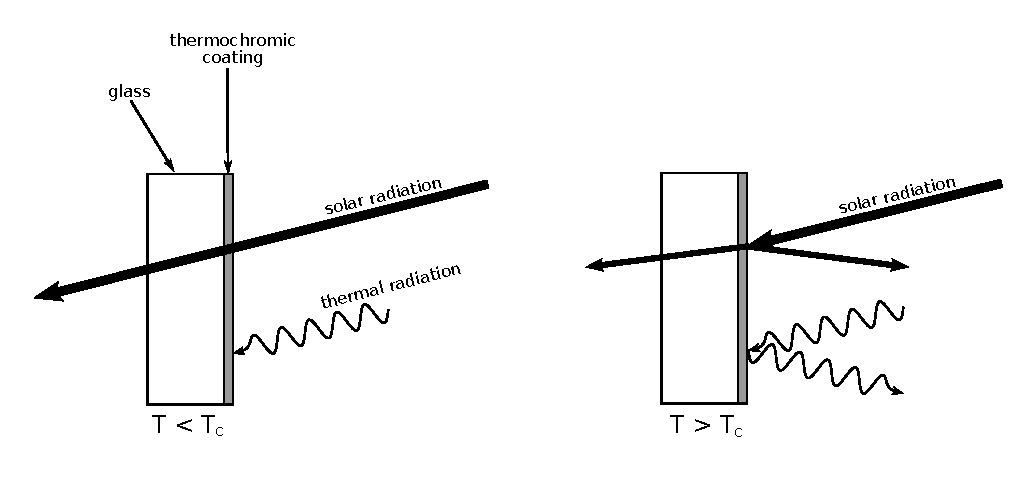
\includegraphics[width=0.5\textwidth]{Figures/TCcoating.pdf}
   \caption{Schematic demonstration of the application of thermochromic materials to advanced window glazing [8].
   In the article it is used as a pictorial representation of how vanadium(IV) oxide thin film will work as 
   an intelligent window. }
\end{figure}


\clearpage
\begin{thebibliography}{9}

      \bibitem{opticalProperties}
      D. Bedeaux, J. Vlieger, 
      \emph{Optical Properties of Surfaces}, 
      Imperial College Press, 
      London, 2001

      \bibitem{intelligentWindows}
      Parkin IP, Manning TD.
      \emph{Intelligent thermochromic windows}, 
      Journal of Chemical Education,
      London 2006;83(3):393. ?I DON'T KNOW WHAT 393 is!? what is it?


      \bibitem{TCcommercialProducts}
      White MA, LeBlanc M.
      \emph{Thermochromism in Commercial Products}, 
      Journal of Chemical Education,
      Canada, September 1999;76(9) ?IS THIS RIGHT? IS SOMETHING WRONG? DO I MISS SOMETHING?!

      \bibitem{TCqualitativeDescription}
      Hiltunen J, Silfsten P, Jaaskelainen T, Parkkinen JPS,
      \emph{A Qualitative Description of Thermochromism in Color Measurements}, 
      ???????????????,
      ???????????????
      
      %\bibitem{Kamalisarvestani2013}
      %Kamalisarvestani M, Saidur R, Mekhilef S, Javadi FS,
      %\emph{Performance, materials and coating technologies of thermochromic thin films on smart windows}, 
      %Renewaable and Sustainable Energy Reviews 26 (2013) 353-364 ???????/????????   Elsevier?
      %Kuala Lumpur, Malaysia 2013; ???????????+

\end{thebibliography}


%
\newpage
\section{\textbf{Book Notes}}
\section{Handbook of Optial Constants of Solids; Edward D. Palik}
Institute for physical Science and Technology, University of Maryland\\
Academic Press 1998, 1985.\\

\subsection{Bulk and thin-film effects; effective-medium theory; p.104}
\begin{itemize}
\item p. 105:\\
   In this discussion, we assume that the characteristic dimensions of the microstructure
   are large enough ($>/\sim 10-20 $Å) so that the individual regions retain essentially their bulk dielectric
   responses, but small ($>/\sim$ 0.1-0.2 $\lambda$) compared to the wavelength of light.
   Then, the macroscopic $\boldsymbol E$ and $\boldsymbol H$ fields of Maxwell's equations will not vary
   appreciably over any single region, and quasistatic theory can be used. This avoids complications
   due to scattering and retardation effects that are dominant in macroscopiccally inhomogeneous 
   systems \cite{Beckmann1968}.
   \\
   \\
   The dielectric functions is obtained from the macroscopic average electric field $\boldsymbol E$ and 
   polarization $\boldsymbol P$ according to
   \begin{align}
      \boldsymbol D &= \varepsilon \boldsymbol E = \boldsymbol E+ 4\pi \boldsymbol P \\
      \boldsymbol P &= \frac{1}{V} \sum q_i \Delta\! \boldsymbol{x_i},
   \end{align}
   where $\Delta \! \boldsymbol{x_i}$ is the displacement of the charge $q_i$ under the action of the 
   local field at $q_i$. It is the apperance of the volume normalizing factor in the latter equation
   that is responsible for the sensitivity of $\varepsilon$ to density.
   \item 
\end{itemize}

\begin{thebibliography}{9}
      \bibitem{Beckmann1968}
      Beckmann P.
      The depolarization of electromagnetic waves.
      Golem, Boulder, Colorado, 1968.

\end{thebibliography}


\subsection{Jensen B: The Quantum Extension of the Drude-Zener Theory in Polar Semiconductors; p.169-188}
p.169-170:\\
\textbf{Introduction}\\
The classical Drude model for the complex dielectric constant of a semi-conductor can be used to
extrct the mobility and the free-carrier density $n_e$ from an analysis of the reflectivity and transmittance
data in the ar infrared (1-4)=
      \cite{Palik1979, Holm1977,Perkowitz1971,Perkowitz1974,Fan1967}.
The dielectric constant $\varepsilon$ is the square of the complex refractive
index, which determines the optical properties of a given material. One has
\begin{align}
   \varepsilon = \varepsilon_1 - i \varepsilon_2 = N^2,
   \label{compEps}
\end{align}
were the real and imaginary parts of the complex  parts of the complex dielectric constant $\varepsilon_1$ 
and $\varepsilon_2$ are functions of the complex refractive index N as
\begin{align}
   N = n -i k
\end{align}
\begin{align}
   \varepsilon = n^2 - k^2
\end{align}
\begin{align}
   \varepsilon = 2nk = \frac{4\pi \sigma}{\omega}
   \label{imEps}
\end{align}
The choice of $n-ik$ rather than $n+ik$ is determiend by the original use of 
$\exp i(\omega t - \boldsymbol q \cdot \boldsymbol r)$ in the assumed plane-wave solution of
Maxwell's equations.
In Eqs \eqref{compEps}-\eqref{imEps}, $n$ is the real part of the complex refractive index, $k$
the imaginary part or extinction coefficient, and $\sigma$ the optical conductivity. The
absorption coefficient $\alpha$ is proportional to $\sigma$, to $\varepsilon_2$, and to $k$:
\begin{align}
   n\alpha = \frac{4 \pi \sigma}{c} = \frac{\omega}{c} \varepsilon_2
\end{align}
\begin{align}
   n\alpha =  = \frac{\omega}{c}k = \frac{1}{\delta}
\end{align}
The extinction coefficient k is essentially the ratio of the free-space wavelength of light of 
frequency $\omega$ to the skin depth $\delta$.\\
%
The Drude theory gives the free-carrier contribution to $\varepsilon_1$ and $\varepsilon_2$ in terms
of the plasma frequency $\bar\omega_p$ and the electron scattering time $\tau$ as
\begin{align}
   \varepsilon_1 &= \varepsilon_{\infty} \frac{1 - \bar\omega_p^2}{\omega^2 \eta}\\
   \label{eps1Drude}
\end{align}
\begin{align}
   \varepsilon_2 &= \frac{\omega_p^2}{\omega^2 \eta} \frac{ 1 }{ \omega \tau}
\end{align}
where $\varepsilon_{\infty}$ is the high-frequencylattice dielectric constant The reail and imaginary
parts of the complex refractive index are obtained from $\varepsilon_1$ and $\varepsilon_2$.
One has
\begin{align}
   \varepsilon &= \sqrt{\varepsilon_1^2 + \varepsilon_2^2} = n^2 + k^2, \\
   n = \sqrt{\frac{\varepsilon + \varepsilon_1}{2} },
   k = \frac{\epsilon_2}{2n} = \sqrt{ \frac{\varepsilon - \varepsilon_1}{2}}.
\end{align}
Experimentally, $n$ and $k$ are found from measurements of the reflectivity R of a bulk, opaque sample
and the transmittance T of a slab, which are given in terms of $n$ and $k$ as
\begin{align}
   R &= \frac{(n-1)^2 + k^2}{(n+1)^2 + k^2} \\
   R &= \frac{ (1-R)^2 e^{-2\omega k d / c} }{ (1-R)^2 e^{-4\omega k d / c} },
\end{align}
where $d$ is the sample thickness. For the slab multiple-reflection effects are averaged,
so that interface fringes are not resolved.
\\
\\
p.171:\\ In the far infrared, for photon energues small compared with $k_0 T$ ($k_0$ boltzmans const.)
and with the energy $\hbar \omega_Q$ of the phonon involved in the scatteering, the
quantum result reduces to the $\lambda^2$ dependenve given by the Drude Theory, and the quasi classical
Boltzmann transport equation (1-3). The departurs from the Drude theory
at high frequencies are associated mainly with $k$ rather than $n$, and hence,
the transmission is affected more than the reflectivity. The latter depends on
$k$ in the region of the reflectivity minimum, where $n \simeq 1$, but is determined 
essentially by $n$ over the region of the absorption spectrum for which $n > k$,
which is the region where departures from the Drude theory would occur.
\\
(...)
\\
The response of electrons to a driving field may be followed from the wuasi-classical
limit of small $\omega$ to the quantum limit that occurs when $\hbar \omega$ is no longer small
compared with characteristic energies of the system. In this case, a generalized Boltzmann equation
is obtained that reduces to the quasi-classical Boltzmann transmport equation when the electron wave 
vector $q$ tends to zero and $\omega$ is small (14-17)=
\cite{Jensen1975,Price1966,Argyres1961,Kohn1958}
. When $\omega$ is appreciable, one obtaines,
under certain conditions, a solution of the Boltzmann equation in terms of a frequency-dependent
relaxation time. This relaxation rate, which has been tabulated as a function of frequency and 
carrier concentration for various materials (18-20)=
\cite{Jensen1977,Jensen1979,Jensen1981}
, can be used in the usual expression of the 
classical Drude theory to obtain the quantum result. In particular, the low-
frequency $\hbar\omega \simeq k_0T$ limit gives a good estimate for the dc mobility as a function
of carrier concentration. At high frequencies, in lightly doped materials in which
polar scattering dominates, $n\alpha$ is proportional to $\lambda^3$ and $\varepsilon_2$ and $k$
are proportional to $\lambda^4$ rather than $\lambda^3$. The real part of the dielectric constant
is givn approximately by the Drude-theory expression and $n \simeq \sqrt{\varepsilon_{\infty}}$
for $\bar\omega_p \ll \omega \ll G/\hbar$, where $G/\hbar$ is the frequency of the fundamental absorption
edge and $G$ is the direct-band-gap energy of the semiconductor. As $\omega$ approaches $G/\hbar$ there
is a small quantum-mechanical correction to $\varepsilon_1$ and hence to $n$.
A summary of the results of the quantum theory is given in Section II.
\\
\\
p.176:\\
\textbf{Comparison with experimental data}\\
A calculation of $\varepsilon_1$ appropriate to electrons in polar semiconductors with the
band structure of the Kane theory and based on the quantum density-matrix equation of motion yields a 
high frequency modification to Eq.\eqref{eps1Drude}. 
For $\omega \tau \gg 1$ and $X < 0.1$, ($X = \hbar \omega/G$) one obtains (18,22)
\begin{align}
   \varepsilon_1 &= \Bigg[ \frac{\varepsilon_{\infty}}{1 - X} \Bigg]\big[ 1 - (X/\varepsilon_{\infty}) - \bar\omega_p^2/\omega^2 \big] \\
                &= \Bigg[ \frac{\varepsilon_{\infty}}{1 - X} \Bigg]\big[ 1 - \bar\omega_p^2/\omega^2 \big] \\
                &= \varepsilon_{\infty}(1 - \bar\omega_p^2/\omega^2), \:\:\:\:\: X \ll 1
\end{align}
We note that $1/\varepsilon_{\infty} <\sim$ 0.1 and hence $X/\varepsilon \ll 1$, for compounds we 
consider, and this term can be neglected. In the limit $X \ll 1$, the quasi-classical high-frequency
Drude result is recovered, as required. For $X \sim 0.1$, there is a high-frequency correction given by
Eq.(some equation), which is used to calculate the numerical values of $\varepsilon_1 = n^2 - k^2$.
The major modification of the classical result is dispersion in $n$ as one approaches the fundamental
absorption edge \cite{Jensen1983}.


\begin{thebibliography}{9}
      \bibitem{Palik1979}
       Palik ED, Hold RT.
       Nondestructire evaluation of semiconductor materials and devices.
       Plenum 1979 (Chap. 7) 
      \bibitem{Holm1977}
         Holm RT, Gibson, Palik ED, 
         J. Appl.Phys. 48,212 (1977)
      \bibitem{Perkowitz1971}
         Perkowitz S. J.Phys.Chem.Solids 32, 2267 (1971)
      \bibitem{Perkowitz1974}
         Perkowitz S, Thorland RH, Phys.Rev. B9, 545 (1974)
      \bibitem{Fan1967}
         Fan HY.
         Semiconductors and semimetals.
         (R.K. Willardson and A.C. Beer eds.),
         Vol.3, Academic Press, New York 1067

      \bibitem{Jensen1975}
         Jensen B. Ann. Phys. 95,229 (1975).
      \bibitem{Price1966}
         Price PJ. IBM J. Res. Dev. 10,395(1966)
      \bibitem{Argyres1961}
         Argyres PN, J. Phys.Chem.Solids 19, 66 (1961)
      \bibitem{Kohn1958}
         Kohn W, Luttinger JM.
         Phys. Rev. 108, 590 (1957)
         Kohn W, Luttinger JM.
         Phys.Rev.109,1892(1958)

      \bibitem{Jensen1977}
         Jensen B. Phys. StatusSolidi. 86, 291 (1978);
         Jensen B. SolidState commun. 24, 853 (1977)
      \bibitem{Jensen1979}
         Jensen B. J. Appl Phys. 50, 5800 (1979)
      \bibitem{Jensen1981}
         Jensen B.
         Laser Induced damage in optical materials; 1980 (H.E. Bennet, A.J. Glass, A.H. Guenther,
         and B.D.Newman, eds.), p.416, National bureau of standards special
         publication 620, Boulder, Colorado, 1981.

      \bibitem{Jensen1983}
         Jensen B, IEEE J. 
         Quantum Electron. QE-18, 1361 (1982); 
         %
         Jensen B, Torabi A, IEEE J.Quantum Electron. QE-19, 448-457,877-882,1362-1365 (1983);
         %
         Jensen N, Torabi A, J.Appl.Phys. 54,2030-2035,3623-3625,5945-5949 (1983).
\end{thebibliography}





\subsection{Shashanka S. Mitra \\
Optical properties of nonmetallic solids for photon energies below the fundamental band gap}
Department of electrical engineering, University of Rhode Island.
\\
\\
p.263-267:\\
\textbf{Infrared Dispersion by plasmons}\\
In the preceeding discussion of absorption of infrared radiation by phonons in a solid, it was tacitly
assumed that the solid was an insulator. This assumption does not hold well for a narrow--gap semiconductor at
ordinary temperatures or for a doped semiconductor with a partially filled conduction or valence band.
The collective excitation of this free-carrier electron gas(plasma) in such a crystal will modify the
infrared absorption by phonons, as discussed earlier. The dispersion mechanism through which electromagnetic
radiation interacts with a solid should include the contribution of free-charge carriers in solids for which
their numbers are significant, in addition to contributions from bound electrons and phonons.
The dielectric response function of such a solid can now be written as 
\begin{align}
   \varepsilon = 1 + 4\pi(\chi_{BE} + \chi_L + \chi_{FC}),
\end{align}
where $\chi_{BE}, \chi_L$ and $\chi_{FC}$, respectively represent the bound electron,lattice,and
free-carrier contributions to the electrical susceptibility. For the spectral region of interest, we
are not concerned with teh bound-electron dispersion; thus this term, as usual, will be 
represented by a dispersion-free, high-frequency dielectric-constant term
\begin{align}
   \varepsilon_{\infty} = 1 + 4\pi \chi_{BE}.
\end{align}
An approximate expression for the dielectric response function for a free-electron gas in a solid can be
obtained from the classical Drude model in which a free electron of effective mass $m*$ and charge $e$
is displaced by an amound $\boldsymbol x$ as a result of interaction with the electric field 
$\boldsymbol E$, with the equation of motion
\begin{align}
   m* \ddot{\boldsymbol x} + m* \gamma \dot{\boldsymbol x} = e \boldsymbol E_0 e^{-i\omega t}
\end{align}
The damping term proportional to the velocity obviously represents the electron-phonon scattering in 
a phenomenological manner. Solving for $\boldsymbol x$, one obtains
\begin{align}
   \boldsymbol x = -e \boldsymbol E /m* \omega (\omega + i \gamma)
\end{align}
The polarization, defined as the electric-dipole moment per unit volume, is given by
\begin{align}
   \boldsymbol P = Ne \boldsymbol x,
\end{align}
where N is the carrier concentration. Recalling that 
\begin{align}
   \boldsymbol P =  \big[ (\varepsilon - 1)/ 4\pi \big] \boldsymbol E,
\end{align}
one readily obtains
\begin{align}
   \varepsilon_{FC} = \varepsilon_{\infty} - \frac{4 \pi N e^2}{m*\omega(\omega + i \gamma)}
\end{align}
for the dielectric response function due to a single-component plasma. In terms of the plasma frequency
defined as 
\begin{align}
   \omega_p = \sqrt{\frac{4\pi N e^2}{\varepsilon_{\infty} m*}}
\end{align}
$\varepsilon_{FC}$ becomes
\begin{align}
   \varepsilon_{FC} = \varepsilon_{\infty} \big[ 1 - \big(\omega_p^2/\omega(\omega + i \gamma)\big)\big].
\end{align}
For a number of semiconductors there exists a region of the infrared spectrum in which the free-carrier 
contributions dominates, and both the bound electron and lattice contributions to dielectric response
function are negligible. For a semiconductor, such a situation prevails in a region of the infrared
spectrum in which $\omega_g \ll \omega_p \ll \omega_{TO}$, where $\hbar \omega_g$ is the
electronic band gap. The analysis of optical response is also smpler in a region in which the reflection


\begin{thebibliography}{9}
      \bibitem{yy}
\end{thebibliography}

\end{document}


